\section{In McCormick's physical model}\label{sec:mcc}

McCormick's current calculation~\cite{McC2} replaces the single collision rate by six energy groups per flavour, with weak rates for plasma scattering and for neutrino self-scattering. This section reads that model in the two-rate language of Section~\ref{sec:link}, and runs the one simulation that decides what self-scattering does.

\paragraph{His collision term is the flux--shear link, exactly, with his archived target.} For one energy group the collision term of his Eq.~(C3), with his default target, isotropy in each group's own frame to first order, is $A\kappa_e(\varepsilon/4\pi-I)+A\kappa_n(\varepsilon/4\pi+c\mu-I)$, with $c$ the dipole coefficient fixed by the group's flux. On his 32 angle bins, with $P_0$ and $P_1$ the projections onto $1$ and $\mu$ (orthogonal because the bins are symmetric), it is
\begin{equation}
C=-\kappa_e(I-P_0)-\kappa_n(I-P_0-P_1)=-\operatorname{diag}(0,\ \kappa_e,\ \kappa_e+\kappa_n,\ \kappa_e+\kappa_n,\ \dots)
\end{equation}
in the discrete orthonormal Legendre basis: plasma drag on the dipole, self-scattering on the shear and above. This is the split link with $\kappa_1=\kappa_e$, $\kappa_2=\kappa_e+\kappa_n$, $r=1+\kappa_n/\kappa_e$, and its connection energy is $k^2(\kappa_e^2/3+4\kappa_n^2/15)$ in the continuum (Appendix~A.13). Taken straight from his compiled right-hand side, the operator matches the diagonal to $3.6\times10^{-15}$, its $\kappa_n$ part to $4.9\times10^{-15}$; on the bins the two weights are $c_0^2=\tfrac13-\Delta\mu^2/12$ and $c_1^2=\tfrac4{15}(1-\Delta\mu^2)$, verified to machine precision at $N_\mu=32$, $64$, $128$ and $1024$ \grade{derived; measured}. Only the plasma term hands momentum to the plasma. The identity is for this default target, the one behind his archived thresholds, which keeps each group's own flux. His boosted option, an isotropic distribution in one neutrino rest frame shared by all groups, $I\propto(1-v\mu)^{-4}$~\cite{McCcode}, ties every group's dipole to a common velocity and is outside the identity; it is the positive common-frame target used in the recorder runs below.

\paragraph{Where his rates sit.} Along his background, $r=1+\kappa_n/\kappa_e$ is nearly constant in time and energy: $2.43$--$2.45$ for $\nu_e$ and $7.69$--$7.77$ for $\nu_{\mu,\tau}$ between $T_b=0.3$ and $5$\,MeV. Inside the collapse, recorded at $r=r_m$ through the readout epoch $1.7\le\epsilon\le4$, the dominant group has $r=7.9$--$8.6$ at $T_H=1$\,MeV and $8.2$--$12.2$ at $T_H=0.51$\,MeV, link rapidity $1.03$--$1.25$, against the admissible window's upper edge $0.20$ \grade{measured}. His physical model lives far outside the window where the rate was measured, and at readout both rates are below $H$ ($\kappa_e/H\approx0.02$--$0.04$, $\kappa_n/H\approx0.16$--$0.27$ at $T_H=1$\,MeV): a large link rapidity on a weak link.

\paragraph{What self-scattering does.} His archived thresholds at $T_H=1$\,MeV are $0.519406\pm0.000156$ with self-scattering and $0.526391\pm0.000109$ without; the perfect fluid gives $0.49742$. The instantaneous free-streaming threshold at that mass with the full equation of state was not in his archive; with his code it is $\delta_c^{\rm inst}=0.53313\pm0.00012$ \grade{measured}. Self-scattering does two things at once: it adds $\kappa_n$ to the total isotropy rate, so the neutrinos stay isotropic longer, and it splits the flux from the shear. Two readings were written before the deciding run. In the timing reading only the isotropy history matters; with the flux--shear split removed and the isotropy history unchanged the threshold stays at $0.5194$. In the link reading the frozen law of Section~\ref{sec:link}, with the energy-weighted link rapidity $u_{\rm eff}=0.831$, places the split-free threshold near $0.5204\pm0.0003$.

\paragraph{The deciding run.} In a copy of his solver the self-scattering term targets isotropy in the plasma frame, $\kappa_n(\varepsilon/4\pi-I)$, and its momentum $\kappa_nq$ is handed to the plasma: the flux and every higher moment then relax at $\kappa_e+\kappa_n$ ($r=1$), and the total isotropy history is unchanged. On one frozen group the operator is $-(\kappa_e+\kappa_n)\operatorname{diag}(0,1,1,\dots)$ to $5.3\times10^{-15}$, energy is conserved to $1.5\times10^{-16}$, and the momentum lost by the neutrinos equals the momentum the plasma receives to $1.5\times10^{-14}$; with $\kappa_n=0$ it reproduces his code bit for bit to $\epsilon=0.6$. The bisection ($T_0=10$\,MeV, six groups, $N=300$, $N_\mu=32$) gives
\begin{equation}
\delta_c(r=1)=0.51972\pm0.00009,
\end{equation}
above his self-scattering threshold by $+0.00031\pm0.00018$, and strictly above it, since his $0.5195625$ forms a black hole and here $0.519625$ disperses \grade{measured; Figure~\ref{fig:mcc}}. Against the lines written first this is neither reading: below the link line, just above the timing band. Most of what self-scattering does to the threshold is timing; the flux--shear split carries a real remainder, $+0.0003$ in $\delta_c$, about a third of what the frozen law predicted and $4.5\%$ of the whole self-scattering shift in $G$. The law measured inside $\tfrac34\le r\le\tfrac32$ does not carry linearly to $r\approx8$; there the link's effect on the threshold is weaker than the straight line. The size of the shift alone could not have told the readings apart: with the measured $\delta_c^{\rm inst}$ the frozen law at rate $1.11$ and the timing reading both land inside their kill lines on his self-scattering threshold.

\paragraph{The kept share leads.} With a read-only recorder in his multigroup solver (the intensities identical bit for bit to an unchanged run), his archived threshold edges were run with the positive common-frame target, at $T_H=1$ and $0.51$\,MeV. Both pairs still split, so with that target the thresholds lie in $[0.51925,0.51956]$ and $[0.52475,0.52513]$. At $r=r_m$ the kept-share anisotropy $1-A$, with $A=I_0^2/\lVert I\rVert^2$ on the bins, separates the collapsing run from the dispersing run first, before $\epsilon=3$ at both masses: about $0.85$ in $\epsilon$ before the peak compaction does and $1.2$--$1.3$ before the energy-frame velocity of the neutrino gas, $v_L=2q/[e+P_r+\sqrt{(e+P_r)^2-4q^2}]$ \grade{measured; Figure~\ref{fig:keptshare}}. The gas frame peaks at $v_L\approx0.11$ ($T_H=1$\,MeV) and $0.16$ ($0.51$\,MeV) near $\epsilon\approx3.5$ and turns to infall after $\epsilon\approx5.3$. Part of the kept share's lead may be that it is second order in the anisotropy; whether the lead is causal is what Section~\ref{sec:door} tests, in the single-rate model.

\begin{figure}[t]\centering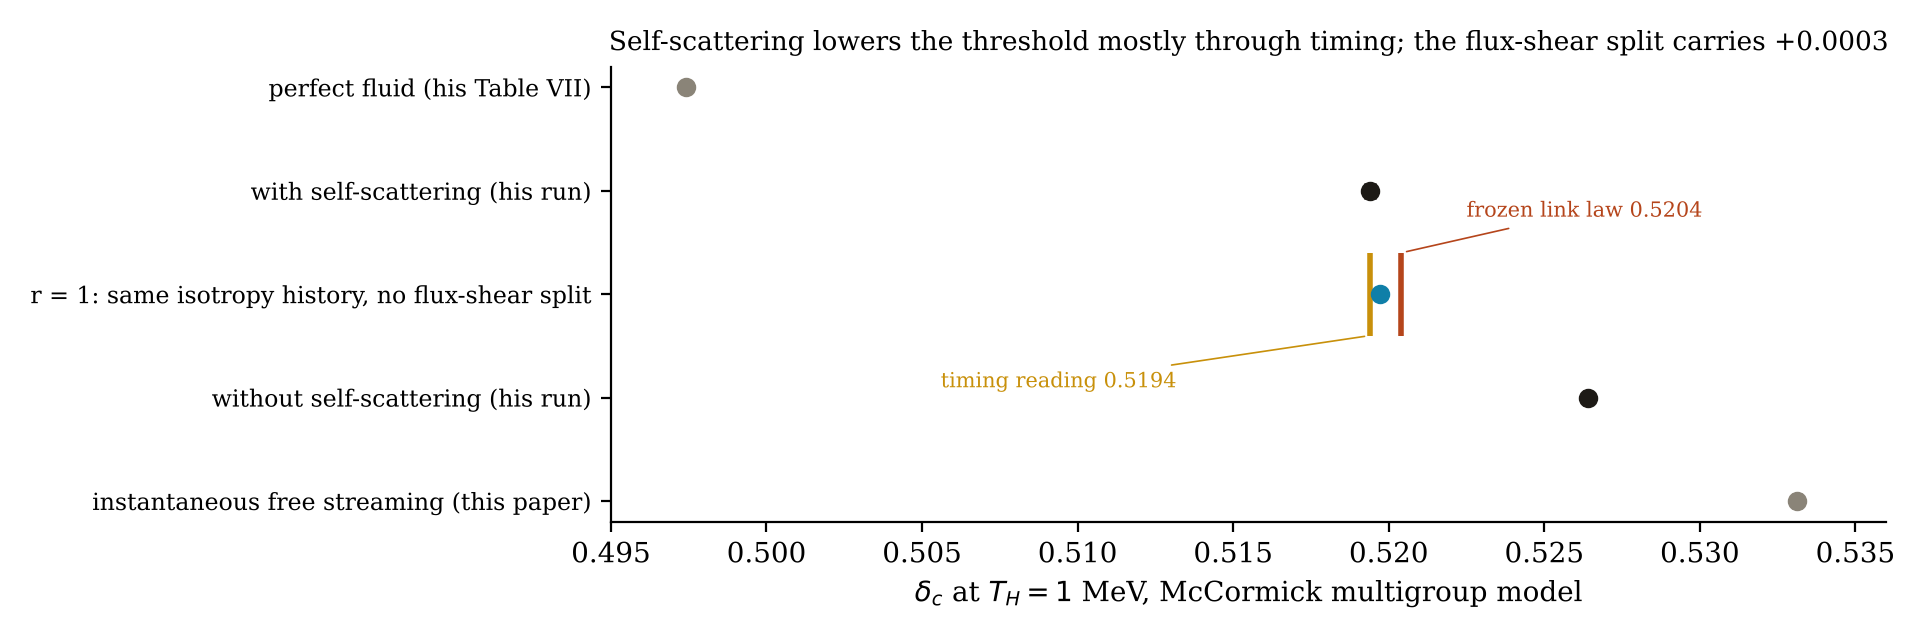
\includegraphics[width=\textwidth]{figs/fig9_selfscatter.png}
\caption{Thresholds at $T_H=1$\,MeV in McCormick's multigroup model. Removing the flux--shear split while keeping the isotropy history ($r=1$) moves the threshold by $+0.0003$ from his self-scattering run; the timing reading predicted no move, the frozen link law $+0.0010$.}\label{fig:mcc}\end{figure}
\begin{figure}[t]\centering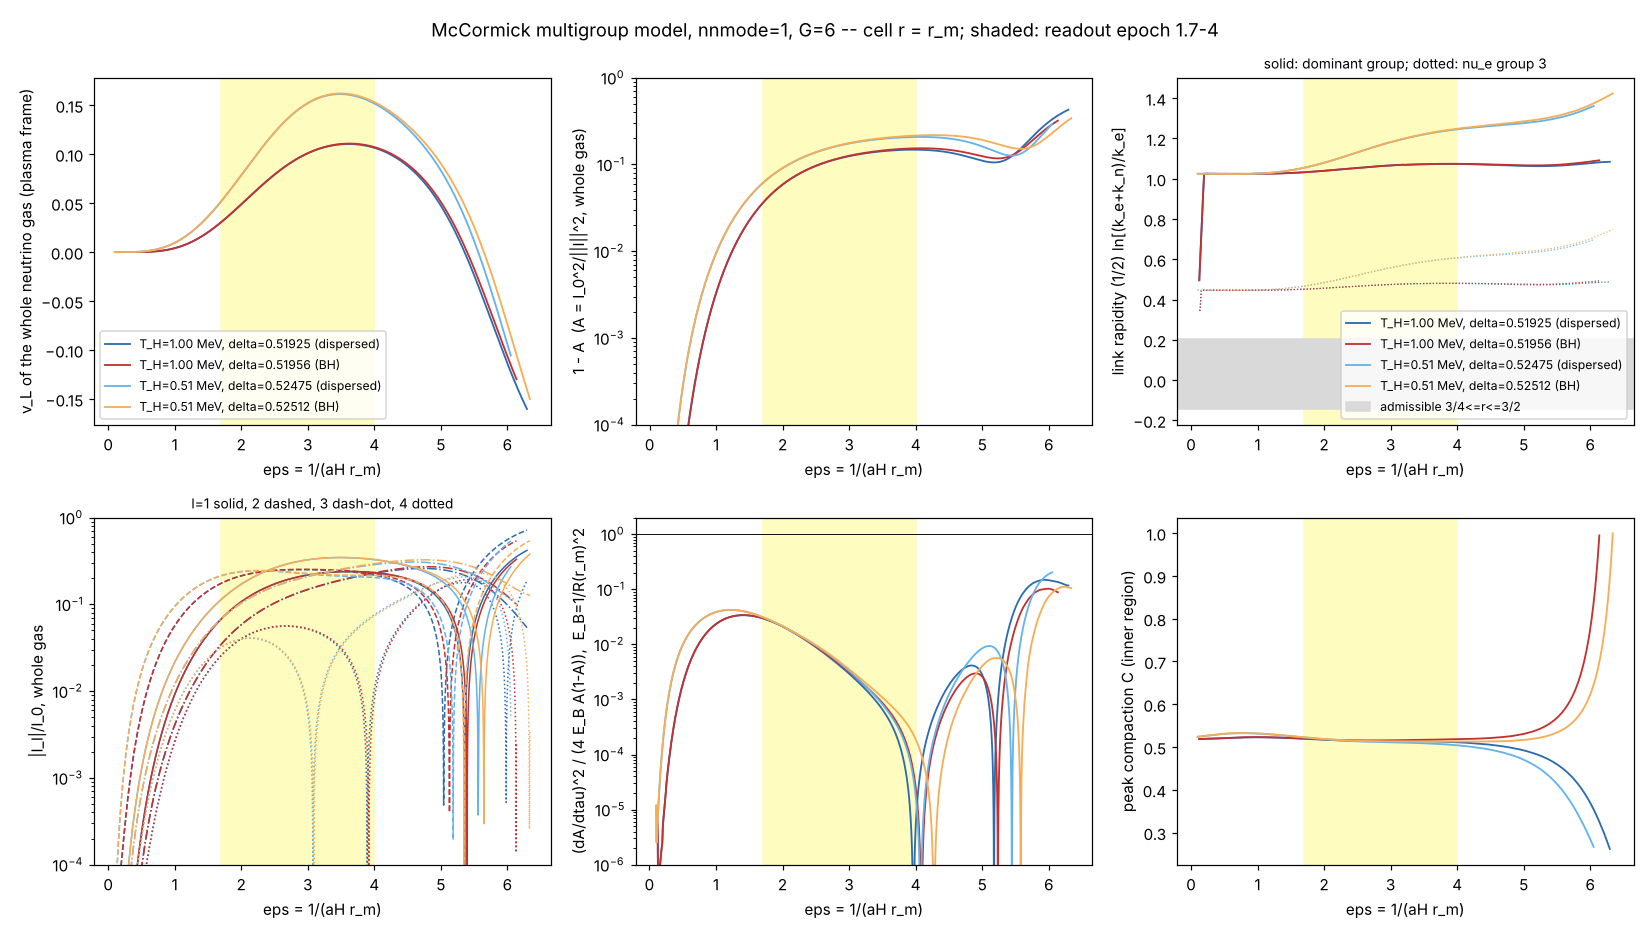
\includegraphics[width=\textwidth]{figs/fig11_keptshare_mcc.png}
\caption{Inside McCormick's multigroup model at $r=r_m$, his archived threshold edges at $T_H=1$ and $0.51$\,MeV (positive common-frame target): energy-frame velocity of the neutrino gas, kept-share anisotropy $1-A$, link rapidity of the dominant and of a $\nu_e$ group against the admissible window (grey), moment ratios, the speed-limit ratio of the kept population, and the peak compaction. The readout epoch $1.7\le\epsilon\le4$ is shaded.}\label{fig:keptshare}\end{figure}
